\documentclass[10pt]{beamer}


% \usepackage{./beamercolorthemeaggie.sty}

\usetheme[progressbar=frametitle]{metropolis}   
\usecolortheme{aggie}

\usepackage{appendixnumberbeamer}
\usepackage{booktabs}
\usepackage[scale=2]{ccicons}
\usepackage{xcolor}
\usepackage{multicol}
\usepackage{float}
\usepackage{csquotes}
\usepackage{subfig}
\usepackage{listings}
\usepackage{pgfplots}
\usepackage{xspace}
\usepgfplotslibrary{dateplot}






% Define C syntax highlighting settings
\lstdefinestyle{customc}{
    belowcaptionskip=1\baselineskip,
    breaklines=true,
    % frame=L,
    xleftmargin=\parindent,
    language=C,
    showstringspaces=false,
    basicstyle=\footnotesize\ttfamily,
    keywordstyle=\bfseries\color{blue!60!black},
    commentstyle=\itshape\color{purple!40!black},
    identifierstyle=\color{black},
    stringstyle=\color{orange},
}
% Define a style for assembly code
% Define a style for assembly code
\lstdefinestyle{asm}{
  language=[x86masm]Assembler,
  basicstyle=\ttfamily\footnotesize,
  commentstyle=\itshape\color{gray},
  keywordstyle=\bfseries\color{black},
  stringstyle=\color{red},
  showstringspaces=false,
  columns=fullflexible,
  keepspaces=true,
  escapechar=§,  % Define an escape character
  morekeywords={.LFB6, .cfi_startproc, pushq, .cfi_def_cfa_offset, 
  .cfi_offset, movq, .cfi_def_cfa_register, movl, pxor, movsd, jmp}
}

\newcommand{\themename}{\textbf{\textsc{metropolis}}\xspace}




%
%   Title
%
\title{HPC Project}
\subtitle{Parallel and Distributed Computing}
\date{\today}
\author{Gabriele Pintus}
\institute{University of Trieste}

\begin{document}

\maketitle

\begin{frame}[fragile]{Introduction}
  \textbf{Assignment 1}: \\
  Measure the latency of multiple collective operations \\
  \textbf{Assignment 2}: \\
  Implement a parallel code which computes the Mandelbrot set
\end{frame}


% First assignment

\section{Assignment 1: \newline \textit{Latency of CoOps}}
\begin{frame}[fragile]{Assignment 1}
    Implement a C code which measures the latency of COOPs.
\end{frame}



% Second assignment

\section{Assignment 2: \newline \textit{The Mandelbrot Set}}
\begin{frame}[fragile]{Assignment 2}
    Implement a hybrid C code which computes the Mandelbrot set using:
    \begin{itemize}
        \item \textbf{OpenMP}: Open Multi-Processing
        \item \textbf{MPI}: Message Passing Interface
    \end{itemize}
\end{frame}

%
%   Mandelbrot Set
%
\begin{frame}[fragile]{Mandelbrot Set}
    Is the set of all complex numbers $c$ for
    which the sequence defined by $z_{n+1} = z_n^2 + c$ does not diverge.
    \begin{figure}[H]
        \centering
        \includegraphics[
            width=0.45\textwidth,
            clip,
            trim=0 35cm 45cm 35cm
        ]{images/mandelbrot_4096x4096_1-min.png}
    \end{figure}
\end{frame}

%
%   Arithmetic Intensity
%
\begin{frame}[fragile]{Arithmetic Intensity}
    Defined as the ratio of the number of arithmetic operations to
    the number of memory operations. \\
    Arithmetic operations:
    \begin{itemize}
        \item 2 mult and 1 add: \texttt{z.x*z.x+z.y*z.y}
        \item 2 mult, 1 sub and 1 add: \texttt{temp=z.x*z.x-z.y*z.y+c.x}
        \item 2 mult and 1 add: \texttt{z.y=2*z.x*z.y+c.y}
        \item 1 add: \texttt{++n}
    \end{itemize}
    Memory operations:
    \begin{itemize}
        \item 1 write: \texttt{int n = 0} 
        \item 2 writes: \texttt{Complex z = \{0,0\}}
        \item 2 reads: \texttt{z.x*z.x+z.y*z.y}
        \item 3 reads and 1 write: \texttt{temp=z.x*z.x-z.y*z.y+c.x}
        \item 3 reads and 1 write: \texttt{z.y=2*z.x*z.y+c.y}
        \item 1 write: \texttt{z.x=temp}
        \item 1 write: \texttt{++n}
    \end{itemize}
\end{frame}
\begin{frame}[fragile]{Arithmetic Intensity}
    The arithmetic intensity is then
    $$
        \frac{11 \cdot N}{ 10\cdot N + 3} 
        = \frac{11}{10+\frac{3}{N}} \xrightarrow{N \to \infty} \frac{11}{10}
        = 1.1 \text{ flops/byte} > 1
    $$
    Compute-bound when the number of iterations is large, i.e. in the light
    and internal regions of the set. \\
    Memory-bound when the number of iterations is small, i.e. in the
    dark external regions of the set. \\
    We are not considering any kind of optimization!
\end{frame}

%
%   OpenMP
%
\begin{frame}[fragile]{OpenMP}
    General purpose API for parallel programming in C, C++ and Fortran.
    Allow to parallelize loops, sections, tasks and more with minimal effort.
    \begin{lstlisting}[language=C, basicstyle=\fontsize{8}{9}\selectfont\ttfamily]
void mandelbrot_set(uint8_t *image) {
    ...
    #pragma omp parallel for schedule(dynamic, CHUNK_SIZE)
    for (int i = 0; i < total_size; ++i) {
        int x = i / HEIGHT;
        int y = i % HEIGHT;
        Complex c = {X_MIN + x * dx, Y_MIN + y * dy};

        // Compute mandelbrot set in the point
        int iter = mandelbrot(c);
        iter = iter % MAX_ITER;

        // store the value
        image[i] = iter;
    }
}
    \end{lstlisting}
\end{frame}
\begin{frame}[fragile]{OpenMP}
    \begin{itemize}
        \item \texttt{\#pragma omp parallel for}: \\
            \quad parallelizes the loop
        \item \texttt{schedule(dynamic, CHUNK\_SIZE)}: \\
            \quad divides the iterations
            in chunks of size \texttt{CHUNK\_SIZE} and assigns \\
            \quad them to threads
            as they become available.
    \end{itemize}
\end{frame}

%
%   Code Optimizations
%
\begin{frame}[fragile,t]{Code Optimizations}
    The following C function \texttt{mandelbrot} computes the Mandelbrot set
    in a given point $c$.
    \begin{lstlisting}[style=customc, basicstyle=\fontsize{8}{9}\selectfont\ttfamily]
int mandelbrot(const Complex c) {
    int n = 0;
    Complex z = {0, 0};
    while ((z.x * z.x + z.y * z.y) < 4 && n < MAX_ITER){
        double temp = z.x * z.x - z.y * z.y + c.x;
        z.y = 2 * z.x * z.y + c.y;
        z.x = temp;
        ++n;
    }
    return n;
}
    \end{lstlisting}
\end{frame}
\begin{frame}[fragile,t]{Code Optimizations}
    Let's cnosider a couple of optimizations:
    \begin{itemize}
        \item \texttt{const Complex c}: the \texttt{const} keyword
        makes the variable \texttt{c} read-only. However, this also
        enables the compiler to pass a pointer to the variable instead of
        copying it.
        \item Magnitude before than \texttt{MAX\_ITER}: for most of the
        points the magnitude of $z$ will be greater than $2$ before reaching
        the maximum number of iterations. Once the first condition is
        false, we don't need to check the second one.
        \item \texttt{++n}: the pre-increment operator is more efficient
        than the post-increment one since it doesn't need to create a temporary
        variable.
    \end{itemize}
\end{frame}

%
%   Compiler's Optimizations
%
\begin{frame}[fragile,t]{Compiler's Optimizations}
    The \textbf{gcc} compiler has an optimization flag \texttt{-O\{0,1,2,3\}} which
    enables several optimizations. We compare the basic code with the
    level 3 optimized one by giving a look at the assembly code. \\
    \begin{itemize}
        \item Less memory accesses
        \item Better data alignment
    \end{itemize}
\end{frame}
%
%   Less Memory Accesses
%
\begin{frame}[fragile,t]{Less Memory Accesses}
    \begin{multicols}{2}
        \begin{lstlisting}[style=asm, basicstyle=\fontsize{6}{7}\selectfont\ttfamily]
movsd	-32(%rbp), %xmm1 # read c.x
movsd	-32(%rbp), %xmm0 # read c.x
mulsd	%xmm1, %xmm0     # c.x * c.x
movsd	-24(%rbp), %xmm2 # read c.y
movsd	-24(%rbp), %xmm1 # read c.y
mulsd	%xmm1, %xmm2     # c.y * c.y
movapd	%xmm0, %xmm1     # c.x * c.x
subsd	%xmm2, %xmm1     # c.x^2 - c.y^2
movsd	-48(%rbp), %xmm0 # read z.x
addsd	%xmm1, %xmm0     # z.x^2 - z.y^2 + c.x
movsd	%xmm0, -16(%rbp) # write z.x
movsd	-32(%rbp), %xmm0 # read c.x
movapd	%xmm0, %xmm1     # c.x
addsd	%xmm0, %xmm1     # c.x + c.x
movsd	-24(%rbp), %xmm0 # read c.y
mulsd	%xmm0, %xmm1     # c.x + c.x * c.y
movsd	-40(%rbp), %xmm0 # read z.y
addsd	%xmm1, %xmm0     # 2 * z.x * z.y + c.y
movsd	%xmm0, -24(%rbp) # write z.y
movsd	-16(%rbp), %xmm0 # read z.x
movsd	%xmm0, -32(%rbp) # write z.x
addl	$1, -4(%rbp)     # write ++n
        \end{lstlisting}

        \columnbreak

        All the memory accesses are unnecessary. The optimized
        code, uses exclusively the CPU registers. \\
        One could manually use \texttt{register}.
        % table - memory accesses
        \begin{table}[H]
            \centering
            \begin{tabular}{cc}
                \toprule
                \textbf{Basic} & \textbf{Optimized} \\
                \midrule
                70 & 20 \\
                \bottomrule
            \end{tabular}
            \caption{Memory accesses}
        \end{table}
        \textbf{ILP} \\
        $-$ pipeline stalls $\rightarrow$ $+$ throughput.
    \end{multicols}
\end{frame}
%
%   Better Data Alignment
%
\begin{frame}[fragile,t]{Better Data Alignment}
    \begin{multicols*}{2}

    %include PNG
    \begin{figure}[H]
        % \centering
        \includegraphics[
            width=0.45\textwidth,
            clip,
            % trim=0 35cm 45cm 35cm
        ]{images/DataAlignmentExample.png}
    \end{figure}
    % \vspace{-10cm}
    \footnotesize{Example of data alignment with a $32$-bit cpu and a cache
    line size of $32$ bytes. When the data is aligned it can be mapped 
    with just one cache line.}
    % The data is the \texttt{MOV [1234h], AX} instruction.

    \columnbreak

    A memory address is said to be $n$-byte aligned if it is a multiple
    of $n$, where $n$ is a power of $2$. \\
    Modern CPUs can access memory by a single memory word at a time,
    which is usually $64$ bits, $128$ bits, $256$ bits. \\
    The amd64 architecture provides sixteen $128$-bit \texttt{xmm0-15} registers
    used for SIMD operations. Two doubles fit in a single register. \\
    By aligning data (\texttt{p2align}), we ensure that \texttt{c.x} and \texttt{c.y}
    are stored in the same memory word.
        
    \end{multicols*}
\end{frame}
\begin{frame}[fragile]{Better Data Alignment consequences}
    Then, the \texttt{movapd} instruction, which can move two packed
    double-precision floating-point values at once, can be used. \\
    Also, when can use the \texttt{mulpd} instruction to perform the two
    multiplications $c.x \cdot c.x$ and $c.y \cdot c.y$ at once. \\
    Nowadays, all CPUs support SIMD instructions, enabling for 
    CPU level parallelism. \\
    Additionally, by aligning data, we optimize the cache usage
    mapping more data in the same cache line. \\
\end{frame}

%
%   Results
%
\begin{frame}[fragile,t]{Results}
    With the \texttt{perf stat} command when can measure several metrics. \\ 
    \begin{table}[H]
        \centering
        \begin{tabular}{cccc}
            \toprule
            \textbf{Metric} & \textbf{Basic} & \textbf{Optimized}\\
            \midrule
            Wall-clock time & 40.53 s & 16.09 s \\
            User time & 316.67 s & 126.71 s \\
            System time & 199.23 ms & 70.34 ms \\
            \hline
            Instructions & 881 billions & 466 billions \\
            Instructions per cycle & 1.11 & 1.29 \\
            \hline
            Cache references & 44.743.584 & 43.485.500 \\
            Cache misses & 0.98\% & 0.34\% \\
            \bottomrule
        \end{tabular}
    \end{table}
    \vfill
    Intel core i7-8550U, 1.8 GHz, 4 cores, 8 threads, 16 GB RAM. \\
    OMP threads: $8$, image size: $2048 \times 2048$.
\end{frame}

%
%   MPI
%
\begin{frame}[fragile,t]{MPI}
    Message Passing Interface is a standard for parallel and distributed
    computing. Communication between processes must be explicitly defined.
    \textbf{Idea}: we want to distribute the load in a dynamic way as
    the OpenMP code does. \\
    \textbf{Solution}: we define a \texttt{MPI\_CHUNK\_SIZE} and we build
    a \textit{work queue}. Each process will get a chunk from the queue
    and will compute it. A new chunk will be assigned to a process
    as it becomes available.
    \newline
    This is a simple, yet effective, way to implement the dynamic scheduler,
    which allows to better distribute the load among the processes.
\end{frame}
\begin{frame}[fragile,t]{MPI - Work Queue}
    The queue data structure, implemented in the \texttt{sys/queue.h} library,
    is built by the root process.
    \begin{lstlisting}[style=customc, basicstyle=\fontsize{7}{7}\selectfont\ttfamily]
    // Create the work queue
    work_queue = (WorkQueue *)malloc(sizeof(WorkQueue));
    TAILQ_INIT(work_queue);

    // Add work items to the queue
    for (uint32_t i = 0; i < n_chunks; ++i){
        WorkItem *item = (WorkItem *)malloc(sizeof(WorkItem));
        item->start_idx = i * MPI_CHUNK_SIZE;
        item->end_idx = (i + 1) * MPI_CHUNK_SIZE;
        if (item->end_idx > total_size)
            item->end_idx = total_size;
        TAILQ_INSERT_TAIL(work_queue, item, entries);
    }
    \end{lstlisting}
\end{frame}
\begin{frame}[fragile,t]{MPI - Communication}
    We use blocking communication to send the chunks to the processes.
    \begin{itemize}
        \item \texttt{MPI\_Send}: sends a message to a process
        \item \texttt{MPI\_Recv}: receives a message from a process
    \end{itemize}
    A further optimization could be to use non-blocking communication
    to overlap computation and communication and reduce the waiting time.
    The root process sends only $2\times4$ bytes, but receive 
    $$2\times4+\texttt{MPI\_CHUNK\_SIZE}\times\texttt{image\_t}$$
    bytes, where \texttt{image\_t} is either $1$ or $2$ bytes.
\end{frame}
\begin{frame}[fragile,t]{MPI - Communication}
    One could decide to use two \enquote{weak} processes, one
    for sending the chunks and one for receiving them. Moreover,
    using non-blocking communication reduce the waiting time. \\
    The worker processes can receive a new chunk immediately after
    finishing the previous one. They don't need to wait for:
    \begin{itemize}
        \item The root process to end its own computation
        \item The root process to copy the previous chunk
        \item The communication to be completed
    \end{itemize}
\end{frame}

%
%   Scaling
%
\begin{frame}[fragile]{Scaling}
    We want to measure the scalability of the code in two ways:
    \begin{itemize}
        \item \textbf{Strong scaling}: we fix the problem size and
        we increase the number of processes. We expect the execution
        time to decrease.
        \item \textbf{Weak scaling}: we increase the problem size
        proportionally to the number of processes. We expect the
        execution time to remain constant.
    \end{itemize}
    In both cases we perform the same test, once by fixing the number
    of MPI processes to 1 and varying the number of OpenMP threads,
    and once by fixing the number of OpenMP threads to 1 and varying
    the number of MPI processes. \\
    Every test is repeated for two problem sizes: $512 \times 512$
    and $4096 \times 4096$.
\end{frame}

%
%   Strong Scaling
%
\begin{frame}[fragile,t]{Strong Scaling}
    We compare the experimental data with the Amdal's law
    given $p=1$.
    \begin{figure}[H]
        \centering
        \resizebox{0.4\textwidth}{!}{
        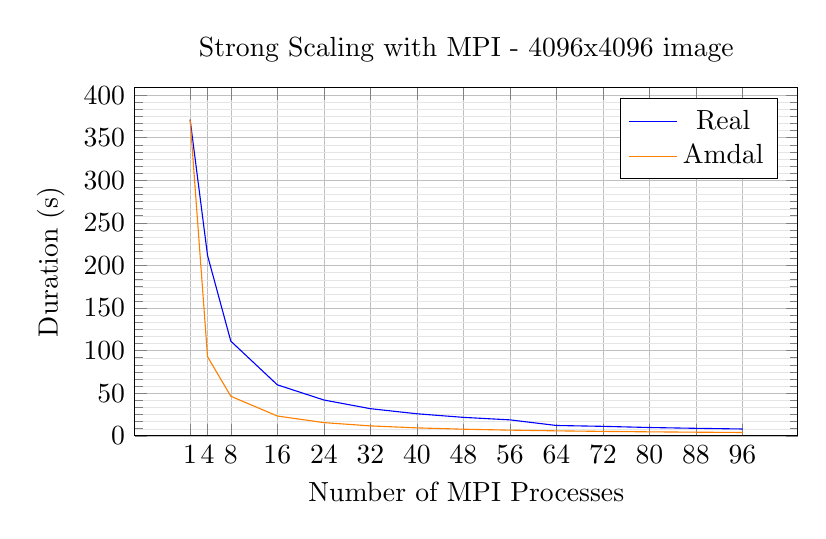
\begin{tikzpicture}
            \begin{axis}[
                title={Strong Scaling with MPI - 4096x4096 image},
                xlabel={Number of MPI Processes},
                ylabel={Duration (s)},
                legend pos=north east,
                grid=both,
                grid style={line width=.1pt, draw=gray!20},
                major grid style={line width=.2pt,draw=gray!50},
                minor tick num=5,
                xtick={1,4,8,16,24,32,40,48,56,64,72,80,88,96},
                % xmode=log,
                % log basis x={2},
                ymin=0,
                % xmin=0,
                % xmax=100,
                ytick={0, 50, 100, 150, 200, 250, 300, 350, 400},
                width=10cm,
                height=6cm,
                % cycle list name=color list,
            ]
            
            % Blue line: Real
            \addplot[
                color=blue,
                mark=none,
                ]
                coordinates {
                (1, 371.358653)
                (4, 211.746975)
                (8, 111.103532)
                (16, 59.841779)
                (24, 42.016501)
                (32, 31.829848)
                (40, 25.848301)
                (48, 21.634139)
                (56, 18.693487)
                (64, 12.088247)
                (72, 11.09093)
                (80, 9.714115)
                (88, 8.76143)
                (96, 7.975981)
                };
                \addlegendentry{Real}
            
            % Orange line: Amdal
            \addplot[
                color=orange,
                mark=none,
                ]
                coordinates {
                (1, 371.358653)
                (4, 92.83966325)
                (8, 46.419831625)
                (16, 23.2099158125)
                (24, 15.473277208333332)
                (32, 11.60495790625)
                (40, 9.283966325)
                (48, 7.736638604166666)
                (56, 6.631404517857143)
                (64, 5.802478953125)
                (72, 5.157759069444444)
                (80, 4.6419831625)
                (88, 4.219984693181818)
                (96, 3.868319302083333)
                };
                \addlegendentry{Amdal}
            \end{axis}
        \end{tikzpicture}
        }
        \resizebox{0.4\textwidth}{!}{
        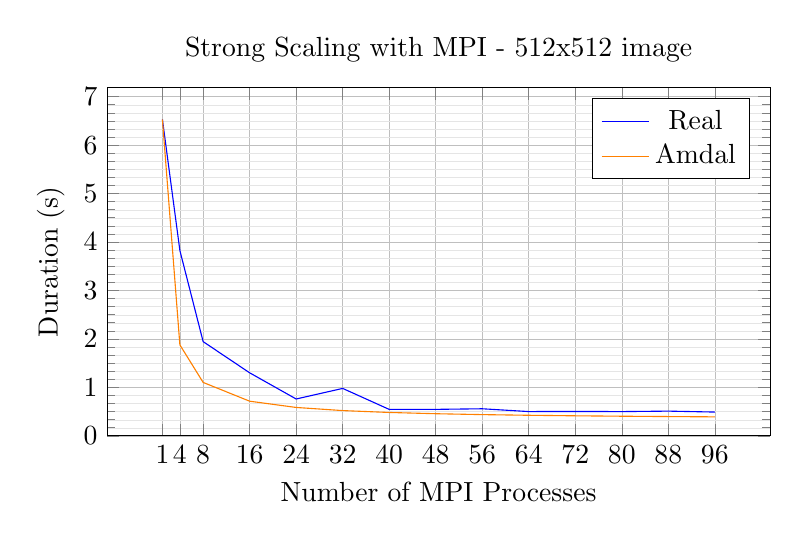
\begin{tikzpicture}
            \begin{axis}[
                title={Strong Scaling with MPI - 512x512 image},
                xlabel={Number of MPI Processes},
                ylabel={Duration (s)},
                legend pos=north east,
                grid=both,
                grid style={line width=.1pt, draw=gray!20},
                major grid style={line width=.2pt,draw=gray!50},
                minor tick num=5,
                xtick={1,4,8,16,24,32,40,48,56,64,72,80,88,96},
                % xmode=log,
                % log basis x={2},
                ymin=0,
                % xmin=0,
                % xmax=100,
                ytick={0, 1, 2, 3, 4, 5, 6, 7},
                width=10cm,
                height=6cm,
                % cycle list name=color list,
            ]
            % real  [6.528405, 3.824648, 1.943719, 1.300054, 0.759538, 0.977942, 0.544757, 0.545445, 0.557732, 0.499887, 0.502379, 0.499451, 0.509071, 0.489834]
            % amdal  [6.528405, 1.8769164375000003, 1.1016683437500003, 0.7140442968750003, 0.5848362812500003, 0.5202322734375003, 0.48146986875000025, 0.4556282656250003, 0.4371699776785717, 0.4233262617187503, 0.4125589270833336, 0.4039450593750003, 0.3968973494318185, 0.3910242578125003]
            % Blue line: Real
            \addplot[
                color=blue,
                mark=none,
                ]
                coordinates {
                (1, 6.528405)
                (4, 3.824648)
                (8, 1.943719)
                (16, 1.300054)
                (24, 0.759538)
                (32, 0.977942)
                (40, 0.544757)
                (48, 0.545445)
                (56, 0.557732)
                (64, 0.499887)
                (72, 0.502379)
                (80, 0.499451)
                (88, 0.509071)
                (96, 0.489834)
                };
                \addlegendentry{Real}
            
            % Orange line: Amdal
            \addplot[
                color=orange,
                mark=none,
                ]
                coordinates {
                (1, 6.528405)
                (4, 1.8769164375000003)
                (8, 1.1016683437500003)
                (16, 0.7140442968750003)
                (24, 0.5848362812500003)
                (32, 0.5202322734375003)
                (40, 0.48146986875000025)
                (48, 0.4556282656250003)
                (56, 0.4371699776785717)
                (64, 0.4233262617187503)
                (72, 0.4125589270833336)
                (80, 0.4039450593750003)
                (88, 0.3968973494318185)
                (96, 0.3910242578125003)
                };
                \addlegendentry{Amdal}
            \end{axis}
        \end{tikzpicture}
        }
    \end{figure}
    \begin{figure}[H]
        \centering
        \resizebox{0.4\textwidth}{!}{
        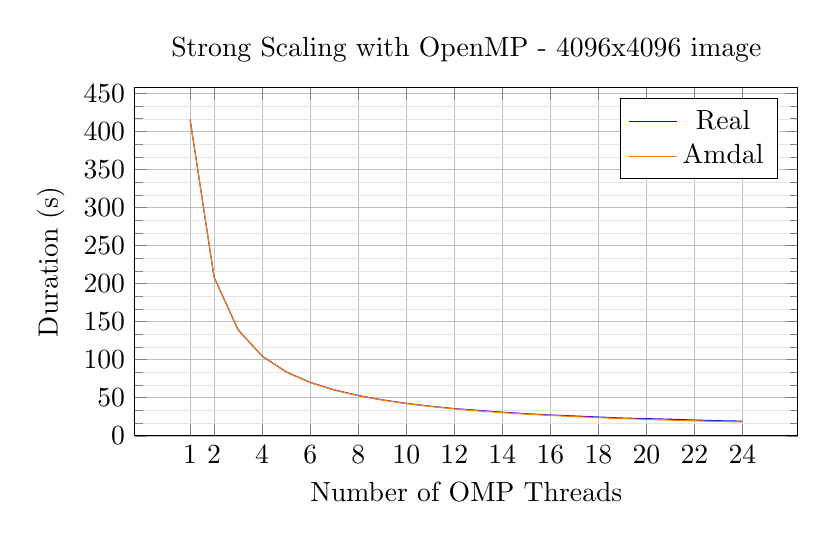
\begin{tikzpicture}
            \begin{axis}[
                title={Strong Scaling with OpenMP - 4096x4096 image},
                xlabel={Number of OMP Threads},
                ylabel={Duration (s)},
                legend pos=north east,
                grid=both,
                grid style={line width=.1pt, draw=gray!20},
                major grid style={line width=.2pt,draw=gray!50},
                minor tick num=2,
                xtick={1,2,4,6,8,10,12,14,16,18,20,22,24},
                % xmode=log,
                % log basis x={2},
                ymin=0,
                % xmin=0,
                % xmax=100,
                ytick={0, 50, 100, 150, 200, 250, 300, 350, 400, 450},
                width=10cm,
                height=6cm,
                % cycle list name=color list,
            ]

            % x = [1, 2, 3, ..., 23, 24]
            % real = [415.661696, 208.247553, 139.165655, 104.656798, 83.975518, 70.16855, 60.33325, 52.92974, 47.198111, 42.618235, 38.863273, 35.710124, 33.33666762346096, 30.927101173999425, 28.976889257945583, 27.276021543253105, 25.985570873724576, 24.62994502459599, 23.28144208948935, 22.47376659569014, 21.729953256477426, 20.643902601709605, 19.759922201114204, 19.208314956723797]
            % amdal = [415.661696, 208.24755299999998, 139.10950533333332, 104.54048149999998, 83.79906719999998, 69.97145766666665, 60.09459371428571, 52.686945749999985, 46.92544177777776, 42.316238599999984, 38.54507236363634, 35.40243383333332, 32.743278153846134, 30.464001857142843, 28.488629066666654, 26.760177874999982, 25.235073882352925, 23.87942588888887, 22.66647768421051, 21.574824299999985, 20.58713790476189, 19.689241181818165, 18.86942243478259, 18.11792191666665]
            
            % Blue line: Real
            \addplot[
                color=blue,
                mark=none,
                ]
                coordinates {
                (1, 415.661696)
                (2, 208.247553)
                (3, 139.165655)
                (4, 104.656798)
                (5, 83.975518)
                (6, 70.16855)
                (7, 60.33325)
                (8, 52.92974)
                (9, 47.198111)
                (10, 42.618235)
                (11, 38.863273)
                (12, 35.710124)
                (13, 33.33666762346096)
                (14, 30.927101173999425)
                (15, 28.976889257945583)
                (16, 27.276021543253105)
                (17, 25.985570873724576)
                (18, 24.62994502459599)
                (19, 23.28144208948935)
                (20, 22.47376659569014)
                (21, 21.729953256477426)
                (22, 20.643902601709605)
                (23, 19.759922201114204)
                (24, 19.208314956723797)
                };
                \addlegendentry{Real}
            
            % Orange line: Amdal
            \addplot[
                color=orange,
                mark=none,
                ]
                coordinates {
                (1, 415.661696)
                (2, 208.24755299999998)
                (3, 139.10950533333332)
                (4, 104.54048149999998)
                (5, 83.79906719999998)
                (6, 69.97145766666665)
                (7, 60.09459371428571)
                (8, 52.686945749999985)
                (9, 46.92544177777776)
                (10, 42.316238599999984)
                (11, 38.54507236363634)
                (12, 35.40243383333332)
                (13, 32.743278153846134)
                (14, 30.464001857142843)
                (15, 28.488629066666654)
                (16, 26.760177874999982)
                (17, 25.235073882352925)
                (18, 23.87942588888887)
                (19, 22.66647768421051)
                (20, 21.574824299999985)
                (21, 20.58713790476189)
                (22, 19.689241181818165)
                (23, 18.86942243478259)
                (24, 18.11792191666665)
                };
                \addlegendentry{Amdal}
            \end{axis}
        \end{tikzpicture}
        }
        \resizebox{0.4\textwidth}{!}{
        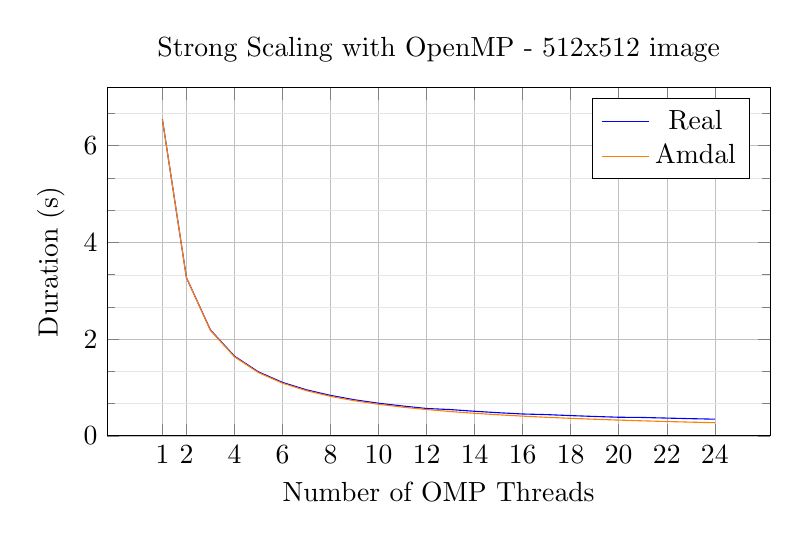
\begin{tikzpicture}
            \begin{axis}[
                title={Strong Scaling with OpenMP - 512x512 image},
                xlabel={Number of OMP Threads},
                ylabel={Duration (s)},
                legend pos=north east,
                grid=both,
                grid style={line width=.1pt, draw=gray!20},
                major grid style={line width=.2pt,draw=gray!50},
                minor tick num=2,
                xtick={1,2,4,6,8,10,12,14,16,18,20,22,24},
                % xmode=log,
                % log basis x={2},
                ymin=0,
                % xmin=0,
                % xmax=100,
                % ytick={0, 50, 100, 150, 200, 250, 300, 350, 400, 450},
                width=10cm,
                height=6cm,
                % cycle list name=color list,
            ]

            % x = [1, 2, 3, ..., 23, 24]
            % real = [6.542253, 3.270055, 2.189338, 1.646339, 1.321695, 1.104557, 0.950666, 0.835814, 0.744772, 0.673606, 0.616551, 0.564914, 0.5420327788647095, 0.507226722269573, 0.47713781646738723, 0.45110666084923023, 0.438131546398441, 0.4178534199562278, 0.3998797734655113, 0.3837668738624881, 0.3793089123223544, 0.366300617912716, 0.35442535450045887, 0.34385476324907194]
            % amdal = [6.542253, 3.2700550000000006, 2.179322333333334, 1.6339560000000009, 1.306736200000001, 1.0885896666666677, 0.9327707142857153, 0.815906500000001, 0.7250121111111122, 0.652296600000001, 0.592802090909092, 0.5432233333333344, 0.501272076923078, 0.4653138571428583, 0.4341500666666678, 0.4068817500000011, 0.38282147058823635, 0.36143455555555665, 0.3422988947368432, 0.3250768000000011, 0.30949490476190583, 0.2953295454545466, 0.2823959565217402, 0.2705401666666678]
            
            % Blue line: Real
            \addplot[
                color=blue,
                mark=none,
                ]
                coordinates {
                (1, 6.542253)
                (2, 3.270055)
                (3, 2.189338)
                (4, 1.646339)
                (5, 1.321695)
                (6, 1.104557)
                (7, 0.950666)
                (8, 0.835814)
                (9, 0.744772)
                (10, 0.673606)
                (11, 0.616551)
                (12, 0.564914)
                (13, 0.5420327788647095)
                (14, 0.507226722269573)
                (15, 0.47713781646738723)
                (16, 0.45110666084923023)
                (17, 0.438131546398441)
                (18, 0.4178534199562278)
                (19, 0.3998797734655113)
                (20, 0.3837668738624881)
                (21, 0.3793089123223544)
                (22, 0.366300617912716)
                (23, 0.35442535450045887)
                (24, 0.34385476324907194)
                };
                \addlegendentry{Real}
            
            % Orange line: Amdal
            \addplot[
                color=orange,
                mark=none,
                ]
                coordinates {
                (1, 6.542253)
                (2, 3.2700550000000006)
                (3, 2.179322333333334)
                (4, 1.6339560000000009)
                (5, 1.306736200000001)
                (6, 1.0885896666666677)
                (7, 0.9327707142857153)
                (8, 0.815906500000001)
                (9, 0.7250121111111122)
                (10, 0.652296600000001)
                (11, 0.592802090909092)
                (12, 0.5432233333333344)
                (13, 0.501272076923078)
                (14, 0.4653138571428583)
                (15, 0.4341500666666678)
                (16, 0.4068817500000011)
                (17, 0.38282147058823635)
                (18, 0.36143455555555665)
                (19, 0.3422988947368432)
                (20, 0.3250768000000011)
                (21, 0.30949490476190583)
                (22, 0.2953295454545466)
                (23, 0.2823959565217402)
                (24, 0.2705401666666678)
                };
                \addlegendentry{Amdal}
            \end{axis}
        \end{tikzpicture}
        }
    \end{figure}
    The OpenMP code scales better, touching the lower bound.
\end{frame}

%
%   Weak Scaling
%
\begin{frame}[fragile,t]{Weak Scaling}
    Theoretically, the execution time should remain constant.
    \begin{figure}[H]
        \centering
        \resizebox{0.4\textwidth}{!}{
        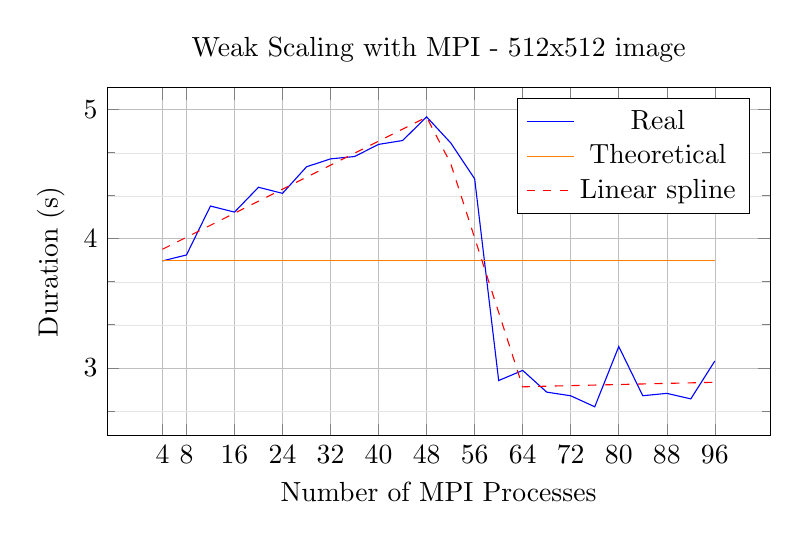
\begin{tikzpicture}
            \begin{axis}[
                title={Weak Scaling with MPI - 512x512 image},
                xlabel={Number of MPI Processes},
                ylabel={Duration (s)},
                legend pos=north east,
                grid=both,
                grid style={line width=.1pt, draw=gray!20},
                major grid style={line width=.2pt,draw=gray!50},
                minor tick num=2,
                xtick={4, 8, 16, 24, 32, 40, 48, 56, 64, 72, 80, 88, 96},
                % xmode=log,
                % log basis x={2},
                % ymin=6,
                % xmin=0,
                % xmax=100,
                % ytick={0, 50, 100, 150, 200, 250, 300, 350, 400, 450},
                width=10cm,
                height=6cm,
                % cycle list name=color list,
            ]

            % x = [4, 8, 12, ..., 96]
            % real = [3.828116, 3.874153, 4.253264, 4.206351, 4.398861, 4.351471, 4.557403, 4.618748, 4.637015, 4.731012, 4.761051, 4.944281, 4.743085, 4.464159, 2.901211, 2.97965, 2.811327, 2.783024, 2.697758, 3.16474, 2.783413, 2.801726, 2.759016, 3.052694]
            % theory = [3.828116, 3.828116, ..., 3.828116]
            % linreg = 3.91816218 4.01124975 4.10433733 4.1974249  4.29051247 4.38360005 4.47668762 4.56977519 4.66286277 4.75595034 4.84903791 4.94212549 4.5835908  4.0064772  3.4293636  2.85225    2.8574569  2.86176193 2.86606697 2.870372   2.87467703 2.87898207 2.8832871  2.88759213]
            
            % Blue line: Real
            \addplot[
                color=blue,
                mark=none,
                ]
                coordinates {
                (4, 3.828116)
                (8, 3.874153)
                (12, 4.253264)
                (16, 4.206351)
                (20, 4.398861)
                (24, 4.351471)
                (28, 4.557403)
                (32, 4.618748)
                (36, 4.637015)
                (40, 4.731012)
                (44, 4.761051)
                (48, 4.944281)
                (52, 4.743085)
                (56, 4.464159)
                (60, 2.901211)
                (64, 2.97965)
                (68, 2.811327)
                (72, 2.783024)
                (76, 2.697758)
                (80, 3.16474)
                (84, 2.783413)
                (88, 2.801726)
                (92, 2.759016)
                (96, 3.052694)
                };
                \addlegendentry{Real}
            
            % Orange line: theory
            \addplot[
                color=orange,
                mark=none,
                ]
                coordinates {
                (4, 3.828116)
                (8, 3.828116)
                (12, 3.828116)
                (16, 3.828116)
                (20, 3.828116)
                (24, 3.828116)
                (28, 3.828116)
                (32, 3.828116)
                (36, 3.828116)
                (40, 3.828116)
                (44, 3.828116)
                (48, 3.828116)
                (52, 3.828116)
                (56, 3.828116)
                (60, 3.828116)
                (64, 3.828116)
                (68, 3.828116)
                (72, 3.828116)
                (76, 3.828116)
                (80, 3.828116)
                (84, 3.828116)
                (88, 3.828116)
                (92, 3.828116)
                (96, 3.828116)
                };
                \addlegendentry{Theoretical}

            % dashed red line: Linear regression
            \addplot[
                color=red,
                mark=none,
                dashed
                ]
                coordinates {
                (4, 3.91816218)
                (8, 4.01124975)
                (12, 4.10433733)
                (16, 4.1974249)
                (20, 4.29051247)
                (24, 4.38360005)
                (28, 4.47668762)
                (32, 4.56977519)
                (36, 4.66286277)
                (40, 4.75595034)
                (44, 4.84903791)
                (48, 4.94212549)
                (52, 4.5835908)
                (56, 4.0064772)
                (60, 3.4293636)
                (64, 2.85225)
                (68, 2.8574569)
                (72, 2.86176193)
                (76, 2.86606697)
                (80, 2.870372)
                (84, 2.87467703)
                (88, 2.87898207)
                (92, 2.8832871)
                (96, 2.88759213)
                };
                \addlegendentry{Linear spline}
            \end{axis}
        \end{tikzpicture}
        }
        \resizebox{0.4\textwidth}{!}{
        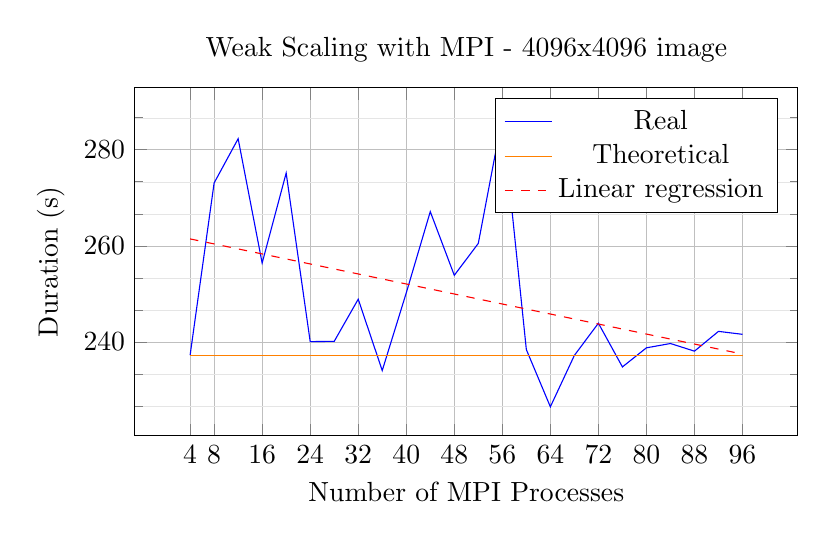
\begin{tikzpicture}
            \begin{axis}[
                title={Weak Scaling with MPI - 4096x4096 image},
                xlabel={Number of MPI Processes},
                ylabel={Duration (s)},
                legend pos=north east,
                grid=both,
                grid style={line width=.1pt, draw=gray!20},
                major grid style={line width=.2pt,draw=gray!50},
                minor tick num=2,
                xtick={4, 8, 16, 24, 32, 40, 48, 56, 64, 72, 80, 88, 96},
                % xmode=log,
                % log basis x={2},
                % ymin=6,
                % xmin=0,
                % xmax=100,
                % ytick={0, 50, 100, 150, 200, 250, 300, 350, 400, 450},
                width=10cm,
                height=6cm,
                % cycle list name=color list,
            ]

            % x = [4, 8, 12, ..., 92, 96]
            % real = [237.225067, 273.079983, 282.287675, 256.41918, 275.142828, 240.061849, 240.118074, 248.890188, 234.048535, 250.200931, 267.119249, 253.859619, 260.50613, 286.838434, 238.399149, 226.496507, 237.196933, 243.889185, 234.796937, 238.769855, 239.666813, 238.076829, 242.194304, 241.577542]
            % theory = [237.225067, 237.225067, ..., 237.225067]
            % linreg = [261.43834089 260.39610037 259.35385984 258.31161931 257.26937879 256.22713826 255.18489773 254.1426572  253.10041668 252.05817615 251.01593562 249.9736951  248.93145457 247.88921404 246.84697352 245.80473299 244.76249246 243.72025194 242.67801141 241.63577088 240.59353035 239.55128983 238.5090493  237.46680877]
            
            % Blue line: Real
            \addplot[
                color=blue,
                mark=none,
                ]
                coordinates {
                (4, 237.225067)
                (8, 273.079983)
                (12, 282.287675)
                (16, 256.41918)
                (20, 275.142828)
                (24, 240.061849)
                (28, 240.118074)
                (32, 248.890188)
                (36, 234.048535)
                (40, 250.200931)
                (44, 267.119249)
                (48, 253.859619)
                (52, 260.50613)
                (56, 286.838434)
                (60, 238.399149)
                (64, 226.496507)
                (68, 237.196933)
                (72, 243.889185)
                (76, 234.796937)
                (80, 238.769855)
                (84, 239.666813)
                (88, 238.076829)
                (92, 242.194304)
                (96, 241.577542)
                };
                \addlegendentry{Real}
            
            % Orange line: theory
            \addplot[
                color=orange,
                mark=none,
                ]
                coordinates {
                (4, 237.225067)
                (8, 237.225067)
                (12, 237.225067)
                (16, 237.225067)
                (20, 237.225067)
                (24, 237.225067)
                (28, 237.225067)
                (32, 237.225067)
                (36, 237.225067)
                (40, 237.225067)
                (44, 237.225067)
                (48, 237.225067)
                (52, 237.225067)
                (56, 237.225067)
                (60, 237.225067)
                (64, 237.225067)
                (68, 237.225067)
                (72, 237.225067)
                (76, 237.225067)
                (80, 237.225067)
                (84, 237.225067)
                (88, 237.225067)
                (92, 237.225067)
                (96, 237.225067)
                };
                \addlegendentry{Theoretical}

            % dashed red line: Linear regression
            \addplot[
                color=red,
                mark=none,
                dashed
                ]
                coordinates {
                (4, 261.43834089)
                (8, 260.39610037)
                (12, 259.35385984)
                (16, 258.31161931)
                (20, 257.26937879)
                (24, 256.22713826)
                (28, 255.18489773)
                (32, 254.1426572)
                (36, 253.10041668)
                (40, 252.05817615)
                (44, 251.01593562)
                (48, 249.9736951)
                (52, 248.93145457)
                (56, 247.88921404)
                (60, 246.84697352)
                (64, 245.80473299)
                (68, 244.76249246)
                (72, 243.72025194)
                (76, 242.67801141)
                (80, 241.63577088)
                (84, 240.59353035)
                (88, 239.55128983)
                (92, 238.5090493)
                (96, 237.46680877)
                };
                \addlegendentry{Linear regression}
            \end{axis}
        \end{tikzpicture}
        }
    \end{figure} % -0.26
    \begin{figure}[H]
        \centering
        \resizebox{0.4\textwidth}{!}{
        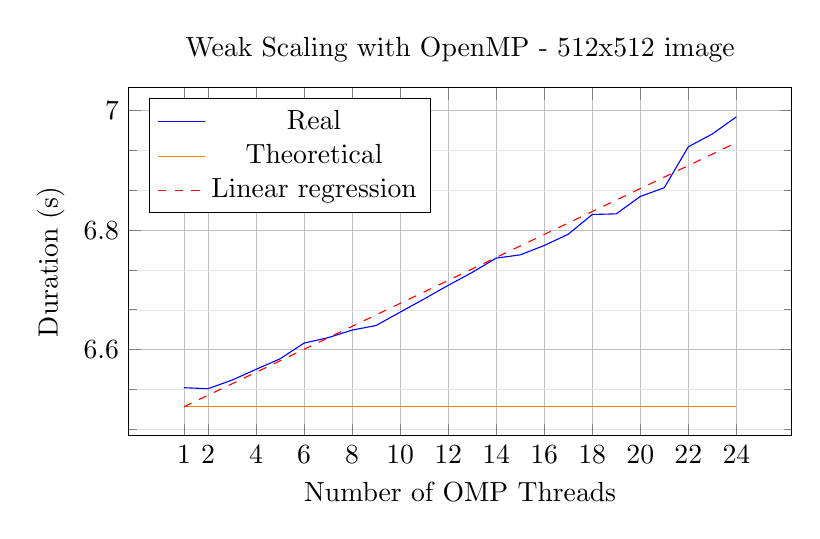
\begin{tikzpicture}
            \begin{axis}[
                title={Weak Scaling with OpenMP - 512x512 image},
                xlabel={Number of OMP Threads},
                ylabel={Duration (s)},
                legend pos=north west,
                grid=both,
                grid style={line width=.1pt, draw=gray!20},
                major grid style={line width=.2pt,draw=gray!50},
                minor tick num=2,
                xtick={1,2,4,6,8,10,12,14,16,18,20,22,24},
                % xmode=log,
                % log basis x={2},
                % ymin=6,
                % xmin=0,
                % xmax=100,
                % ytick={0, 50, 100, 150, 200, 250, 300, 350, 400, 450},
                width=10cm,
                height=6cm,
                % cycle list name=color list,
            ]

            % x = [1, 2, 3, ..., 23, 24]
            % real = [6.535942, 6.534258, 6.548605, 6.566685, 6.584302, 6.610648, 6.619744, 6.632408, 6.640174, 6.662464, 6.684632, 6.707382, 6.729084, 6.753055, 6.758507, 6.77418, 6.793104, 6.826184, 6.827232, 6.856378, 6.871, 6.939576, 6.961086, 6.989746]
            % theory = [6.535942, 6.535942, ..., 6.535942 ]
            % linreg = [6.50395693 6.52320116 6.5424454  6.56168964 6.58093388 6.60017812 6.61942236 6.63866659 6.65791083 6.67715507 6.69639931 6.71564355 6.73488779 6.75413202 6.77337626 6.7926205  6.81186474 6.83110898 6.85035322 6.86959745 6.88884169 6.90808593 6.92733017 6.94657441]
            
            % Blue line: Real
            \addplot[
                color=blue,
                mark=none,
                ]
                coordinates {
                (1, 6.535942)
                (2, 6.534258)
                (3, 6.548605)
                (4, 6.566685)
                (5, 6.584302)
                (6, 6.610648)
                (7, 6.619744)
                (8, 6.632408)
                (9, 6.640174)
                (10, 6.662464)
                (11, 6.684632)
                (12, 6.707382)
                (13, 6.729084)
                (14, 6.753055)
                (15, 6.758507)
                (16, 6.77418)
                (17, 6.793104)
                (18, 6.826184)
                (19, 6.827232)
                (20, 6.856378)
                (21, 6.871)
                (22, 6.939576)
                (23, 6.961086)
                (24, 6.989746)
                };
                \addlegendentry{Real}
            
            % Orange line: theory
            \addplot[
                color=orange,
                mark=none,
                ]
                coordinates {
                (1, 6.50395693)
                (2, 6.50395693)
                (3, 6.50395693)
                (4, 6.50395693)
                (5, 6.50395693)
                (6, 6.50395693)
                (7, 6.50395693)
                (8, 6.50395693)
                (9, 6.50395693)
                (10, 6.50395693)
                (11, 6.50395693)
                (12, 6.50395693)
                (13, 6.50395693)
                (14, 6.50395693)
                (15, 6.50395693)
                (16, 6.50395693)
                (17, 6.50395693)
                (18, 6.50395693)
                (19, 6.50395693)
                (20, 6.50395693)
                (21, 6.50395693)
                (22, 6.50395693)
                (23, 6.50395693)
                (24, 6.50395693)
                };
                \addlegendentry{Theoretical}

            % dashed red line: Linear regression
            \addplot[
                color=red,
                mark=none,
                dashed
                ]
                coordinates {
                (1, 6.50395693)
                (2, 6.52320116)
                (3, 6.5424454)
                (4, 6.56168964)
                (5, 6.58093388)
                (6, 6.60017812)
                (7, 6.61942236)
                (8, 6.63866659)
                (9, 6.65791083)
                (10, 6.67715507)
                (11, 6.69639931)
                (12, 6.71564355)
                (13, 6.73488779)
                (14, 6.75413202)
                (15, 6.77337626)
                (16, 6.7926205)
                (17, 6.81186474)
                (18, 6.83110898)
                (19, 6.85035322)
                (20, 6.86959745)
                (21, 6.88884169)
                (22, 6.90808593)
                (23, 6.92733017)
                (24, 6.94657441)
                };
                \addlegendentry{Linear regression}
            \end{axis}
        \end{tikzpicture}
        }
        \resizebox{0.4\textwidth}{!}{
        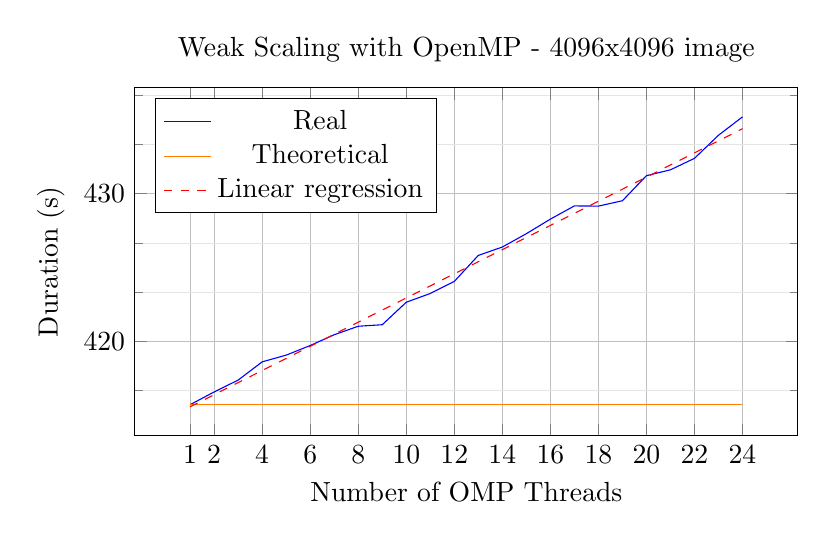
\begin{tikzpicture}
            \begin{axis}[
                title={Weak Scaling with OpenMP - 4096x4096 image},
                xlabel={Number of OMP Threads},
                ylabel={Duration (s)},
                legend pos=north west,
                grid=both,
                grid style={line width=.1pt, draw=gray!20},
                major grid style={line width=.2pt,draw=gray!50},
                minor tick num=2,
                xtick={1,2,4,6,8,10,12,14,16,18,20,22,24},
                % xmode=log,
                % log basis x={2},
                % ymin=6,
                % xmin=0,
                % xmax=100,
                ytick={400, 410, 420, 430, 440, 450},
                width=10cm,
                height=6cm,
                % cycle list name=color list,
            ]

            % x = [1, 2, 3, ..., 23, 24]
            % real = [415.687145, 416.55117, 417.355026, 418.592702, 419.048879, 419.699992, 420.430216, 421.008028, 421.110732, 422.635459, 423.231421, 424.04977, 425.812405, 426.381106, 427.286019, 428.274215, 429.170853, 429.15761, 429.521595, 431.220551, 431.619372, 432.396585, 433.96322, 435.211153]
            % theory = [415.687145, 415.687145, ..., 415.687145 ]
            % linreg = [415.54423536 416.36435701 417.18447866 418.00460031 418.82472196 419.64484361 420.46496526 421.28508691 422.10520856 422.92533021 423.74545186 424.56557351 425.38569516 426.20581681 427.02593846 427.84606011 428.66618176 429.48630341 430.30642506 431.12654671 431.94666835 432.76679 433.58691165 434.4070333 ]
            
            % Blue line: Real
            \addplot[
                color=blue,
                mark=none,
                ]
                coordinates {
                (1, 415.687145)
                (2, 416.55117)
                (3, 417.355026)
                (4, 418.592702)
                (5, 419.048879)
                (6, 419.699992)
                (7, 420.430216)
                (8, 421.008028)
                (9, 421.110732)
                (10, 422.635459)
                (11, 423.231421)
                (12, 424.04977)
                (13, 425.812405)
                (14, 426.381106)
                (15, 427.286019)
                (16, 428.274215)
                (17, 429.170853)
                (18, 429.15761)
                (19, 429.521595)
                (20, 431.220551)
                (21, 431.619372)
                (22, 432.396585)
                (23, 433.96322)
                (24, 435.211153)
                };
                \addlegendentry{Real}
            
            % Orange line: theory
            \addplot[
                color=orange,
                mark=none,
                ]
                coordinates {
                (1, 415.687145)
                (2, 415.687145)
                (3, 415.687145)
                (4, 415.687145)
                (5, 415.687145)
                (6, 415.687145)
                (7, 415.687145)
                (8, 415.687145)
                (9, 415.687145)
                (10, 415.687145)
                (11, 415.687145)
                (12, 415.687145)
                (13, 415.687145)
                (14, 415.687145)
                (15, 415.687145)
                (16, 415.687145)
                (17, 415.687145)
                (18, 415.687145)
                (19, 415.687145)
                (20, 415.687145)
                (21, 415.687145)
                (22, 415.687145)
                (23, 415.687145)
                (24, 415.687145)
                };
                \addlegendentry{Theoretical}

            % dashed red line: Linear regression
            \addplot[
                color=red,
                mark=none,
                dashed
                ]
                coordinates {
                (1, 415.54423536)
                (2, 416.36435701)
                (3, 417.18447866)
                (4, 418.00460031)
                (5, 418.82472196)
                (6, 419.64484361)
                (7, 420.46496526)
                (8, 421.28508691)
                (9, 422.10520856)
                (10, 422.92533021)
                (11, 423.74545186)
                (12, 424.56557351)
                (13, 425.38569516)
                (14, 426.20581681)
                (15, 427.02593846)
                (16, 427.84606011)
                (17, 428.66618176)
                (18, 429.48630341)
                (19, 430.30642506)
                (20, 431.12654671)
                (21, 431.94666835)
                (22, 432.76679)
                (23, 433.58691165)
                (24, 434.4070333)
                };
                \addlegendentry{Linear regression}
            \end{axis}
        \end{tikzpicture}
        }
    \end{figure} % Slope = 0.82
    % As before, the OpenMP code scales better.
\end{frame}





\end{document}